\documentclass{article}
%
%
%	kepler_triangle.tex
%
%	David Meyer
%	dmm613@gmail.com
%	10 May 2024
%
%
%   get various packages
%
\usepackage[margin=1.0in]{geometry}                                     % adjust margins
\geometry{letterpaper}                                                  % or a4paper or a5paper or ... 
\usepackage{url}                                                        % need this to use URLs in bibtex
\usepackage{setspace}                                                   % need this for \setstrech{...}
\usepackage{scrextend}                                                  % need this for addmargin
\usepackage[export]{adjustbox}                                          % need this to get frame for includegraphics
%
%   tikz et al
%
\usepackage{tikz}
\tikzset{>=latex}                                                       % default to LaTeX arrow head
\usetikzlibrary{calc,patterns,angles,quotes,shapes,math,decorations,
                through,intersections,lindenmayersystems,backgrounds,
                hobby,matrix}
\usepackage{tikz-cd}
\tikzcdset{every arrow/.append style={-latex}}                          % commutative diagrams
\usepackage{circuitikz}                                                 % draw circuits    
\usepackage{pgfplots}
%
%	more math stuff
%
\usepackage{amsmath,amsfonts,amssymb,amsthm}
\usepackage{bm}
\usepackage{mathtools}
\usepackage{commath}                                                    % get \norm{x}
\usepackage{fixmath}                                                    % get \mathbold
\usepackage{gensymb}                                                    % get \degree
\usepackage{mathrsfs}
\usepackage{hyperref}
\usepackage{subcaption}
\usepackage{authblk}                                                    % comment out if using beamer (stops \author{} from working in beamer)
\usepackage{graphicx}
\usepackage{hyperref}
\usepackage{alltt}
\usepackage{xcolor}
\usepackage{colortbl}                                                   % \rowcolor{yellow!75} etc
\usepackage{float}
\usepackage{braket}
\usepackage{siunitx}
\usepackage{relsize}
\usepackage{multirow}
\usepackage{esvect}
\usepackage{enumitem}                                                   % use characters instead of numbers in enumerate
\usepackage{changepage}                                                 % needed for \begin{adjustwidth}{-3.25em}{-2.0em} (left justify)
\usepackage{bigints}
\usepackage{multirow}                                                   % \multirow and \multicolumn
%
%	lualatex
%
%	Put this before \documentclass
%
%	!TEX TS-program = LuaLaTeX
%
%
% \usepackage{luatex85,luamplib}
% \mplibnumbersystem{double}
% \mplibtextextlabel{enable}
%
%
%
%	Describe floating point parameters, \fpeval
%
\ExplSyntaxOn
\cs_set_eq:NN \fpeval \fp_eval:n
\ExplSyntaxOff
%
%	Get the x and y components out of a coordinate, e.g.
%
%	\coordinate (EP) at (8,5);
%	\gettikzxy{(EP)}{\slopex}{\slopey}
%
\makeatletter
\newcommand{\gettikzxy}[3]{%
  \tikz@scan@one@point\pgfutil@firstofone#1\relax
  \edef#2{\the\pgf@x}%
  \edef#3{\the\pgf@y}%
}
\makeatother
%
%
%	Watermarks
%
% \usepackage{draftwatermark}
% \SetWatermarkText{Draft}
% \SetWatermarkScale{5}
% \SetWatermarkLightness {0.9} 
% \SetWatermarkColor[rgb]{0.7,0,0}
%
%
%	theorems, definitions, etc
%
\theoremstyle{definition}
\newtheorem{theorem}{Theorem}[section]
\newtheorem{definition}{Definition}[section]
\newtheorem{proposition}{Proposition}[section]
\newtheorem{lemma}{Lemma}[section]
\newtheorem{example}{Example}[section]
\newtheorem{remark}{Remark}[section]
%
%	For drawing matrix products 
%
\newcommand*{\vertbar}{\rule[-1ex]{0.5pt}{2.5ex}}
\newcommand*{\horzbar}{\rule[.5ex]{2.5ex}{0.5pt}}

%
%	The following code allows you to do
%
%	\begin{bmatrix}[r] (or [c] or [l])
%
\makeatletter
\renewcommand*\env@matrix[1][c]{\hskip -\arraycolsep
  \let\@ifnextchar\new@ifnextchar
  \array{*\c@MaxMatrixCols #1}}
\makeatother
%
%	make \arg{min,max}_{n \to \infty} work nicely
%
\newcommand{\argmax}{\operatornamewithlimits{argmax}}
\newcommand{\argmin}{\operatornamewithlimits{argmin}}
%
%	handy commands
%
\newcommand*{\Scale}[2][4]{\scalebox{#1}{$#2$}}
\DeclareMathOperator{\E}{\mathbb{E}}
\DeclareMathOperator{\bda}{\Big \downarrow}						% big down arrow
\newcommand{\veq}{\mathrel{\rotatebox{90}{$=$}}}
%
%	Title, author and date
%
\title{A Few Notes on Kepler Triangles}
\author{David Meyer \\ \href{mailto:dmm613@gmail.com}
                            {dmm613@gmail.com}}
\date{Last Update: \today \\
	 {\vspace{1.00mm} \small Initial Version: May 10, 2024}}
%
%
%
%
\begin{document}
\maketitle
%
%
%
\section{Introduction}
\label{section:introduction}
A Kepler triangle is a right triangle whose sides are related by
a geometric progression
\cite{wiki:geometric_series,wikipedia:kepler_triangle} where the
ratio of the progression is $\sqrt{\phi}$, the square root of the
golden ratio $\phi$ \cite{wiki:golden_ratio}. The Kepler triangle
has sides $1:\sqrt{\phi}:\phi$. The triangle is named after the
famous German astronomer and mathematician Johannes Kepler
\cite{wikipedia:johannes_kepler}.

\bigskip
\noindent
More generally, if the ratio of the geometric progression is
$\sqrt{x}$, then the sides of the triangle are in the ratio $1 :
\sqrt{x} : x$. From this we know (by the Pythagorean theorem
\cite{wiki:trig}) that $1^{2} +(\sqrt{x})^{2} =
x^{2}$. Simplifying we get $1 +x = x^{2}$, or in a more standard
form $x^{2}-x-1 = 0$.  This polynomial turns out to be the
minimal characteristic polynomial of the golden ratio $\phi$, so
we know that $x = \phi$.

\bigskip
\noindent
Interestingly, a triangle with sides $k$, $k\sqrt{x}$, and $kx$
is also a Kepler triangle. This is because the ratio of the sides
of this triangle is $k:k\sqrt{x}:kx$, and if we divide each side
by $k$ we see that the ratio of this triangle's sides is
$1:\sqrt{x}:x$. $\blacksquare$

\bigskip
\noindent
We can also see this by considering following triangle:

\bigskip
%
%       Draw the triangle
%
\begin{figure}[H]                                                               % wrap it in a figure
  \centering                                                                    % center everything
  \resizebox{0.25 \textwidth}{!} {                                              % resize the figure if you like
      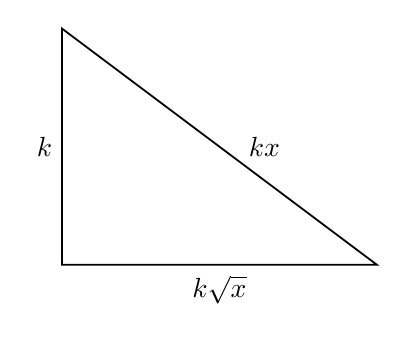
\begin{tikzpicture} 
%
%       Define named points for the vertices of the right
%       triangle
%
        \coordinate (A) at (0,0);
        \coordinate (B) at (4,0);
        \coordinate (C) at (0,3);
%    
%       Draw the right triangle using the named points, adjusting
%		the line width
%
        \draw [line width=0.65pt] (A) -- (B) -- (C) -- cycle;
%
%       Label the edges
%
        \draw [draw=none] (A) -- (B) node [midway,below,yshift=-0.15mm] {$k\sqrt{x}$};
        \draw [draw=none] (A) -- (C) node [midway,left]                 {$k$};
        \draw [draw=none] (B) -- (C) node [midway,right, xshift=0.25cm] {$kx$};
      \end{tikzpicture}
  }                                                                             % end resizebox
\end{figure}                                                                    % done
%
%
%
\noindent 
By the Pythagorean theorem we know that

\vspace{1.50em}
\begin{math}
\begin{array}{rcll} 
(kx)^{2} 
&=& (k\sqrt{x})^{2} + k^{2}
		&\hspace{1.25em} \mathrel{\#} \text{by the Pythagorean theorem} \\
[8pt]
&\Rightarrow& (kx)^{2}- (k\sqrt{x})^{2} - k^{2} = 0 
		&\hspace{1.25em} \mathrel{\#} \text{subtract $\left ( (k\sqrt{x})^{2} + k^{2} \right )$ 
											from both sides } \\
[8pt]
&\Rightarrow& k^2x^2- k^2x - k^{2} = 0 
		&\hspace{1.25em} \mathrel{\#} \text{square terms} \\	
[8pt]
&\Rightarrow& k^{2}(x^{2} - x - 1) = 0 
		&\hspace{1.25em} \mathrel{\#} \text{factor out $k^2$} \\
[8pt]
&\Rightarrow& x^{2} - x - 1 = 0 
		&\hspace{1.25em} \mathrel{\#} \text{divide both sides by $k^2$}
\end{array}
\end{math} 

\bigskip
\noindent
And again, we know that $x^{2} - x - 1$ is $\phi$'s minimal
characteristic polynomial and so $x = \phi =
\frac{1+\sqrt{5}}{2}$ and the ratio of the sides of this triangle
is $1:\sqrt{\phi}:\phi$. $\blacksquare$
%
%
%
\section{Conclusions}
\label{section:conclusions}
%
%
%
\section*{Acknowledgements}
\label{section:acknowledgements}
%
%	LaTeX source on overleaf.com
%
\section*{\LaTeX \hspace{0.025 mm} Source}
\url{https://www.overleaf.com/read/btgfkkdzktbt#adfb58}
%
%	get a bibliography
%
%	Note:.bib files go in ~/Library/texmf/bibtex/bib with TeXShop (MacTeX).
%	You can also use an absolute path, e.g. \bibliography{/Users/dmm/papers/bib/qc}
%
\bibliographystyle{plain}
\bibliography{qc}
%
%
%
% \section*{Appendix A}
%
%	done
%
\end{document} 

